This chapter expands our theoreitcal framework, beginning with an exploration of chiral theories. Because the SM is chiral, this provides the foundation needed to briefly review it in Section \ref{sec:SM}. Motivated by the shortcomings of the SM, we will motivate extenstions in Section \ref{sec:Motiv}, before considering the $\SU(5)$ GUT in Section \ref{sec:SU5} as an example.
\section{Chiral theories} \label{sec:chiral}
To understand the SM, we need to grasp understand \text{chirality}. This attribute of a theory arises from the Dirac equation 
\begin{equation}
    (i\gamma^\mu \partial_\mu - m)\psi (x) =0\;,
\end{equation}
where $\gamma^\mu$ is the gamma matrices. This can be rewritten, by moving to momentum space using the operator $\slashed{p}=\gamma^\mu(i\partial_\mu)$ and working in the Weyl representation, yields the matrix equation
\begin{equation}
\begin{pmatrix}
-m & p^0 - \vec{\sigma} \cdot \vec{p} \\
p^0 + \vec{\sigma} \cdot \vec{p} & -m
\end{pmatrix}
\begin{pmatrix}
\psi_L \\
\psi_R
\end{pmatrix}
= 0\;.
\end{equation}
The equation reveals that for massless particles the left- and right-handed Weyl spinors $\psi_L$ and $\psi_R$ do not mix \cite{Lancaster:2014}. For massless fermions, an additional symmetry also applies for the field, namely the chiral symmetry $\psi\to e^{i\gamma^5\phi}\psi$ \cite{Zee:2010}. 

In a \textit{chiral theory}, like the SM, the left- and right handed fermions transform differently under the gauge group. Consequently, you cannot combine left- and right-handed fermions to form a gauge-invariant mass term in the Lagrangian, such as 
\begin{equation}
    \mathcal{L}_{\text{mass}} = -m\bar{\psi}\psi = -m(\bar{\psi}_L\psi_R + \bar{\psi}_R\psi_L) \;,\label{eq:Chiralmass}
\end{equation}
Thus, in chiral theories, fermions obtain mass via spontaneous symmetry breaking (SSB), as in the Higgs mechanism (see Section \ref{sec:SMHiggs}).

\section{Standard Model} \label{sec:SM} 
Having established the implications of a chiral theory, we will in this section review the core components of the SM and motivate the work of physics beyond the Standard Model (BSM) particularly Grand Unified Theories (GUT)s. 

The SM is governed by two main types of symmetries. The first describes the symmetry of spacetime, which mathematically is described by the Lorentz and Poincaré group. The second of these is the gauge symmetry, which has the semi-simple group structure
\begin{equation}
    \mathcal{G}_{\mathrm{SM}}=\mathrm{SU}(3)_C\times\mathrm{SU}(2)_L\times\mathrm{U}(1)_Y\,,
\end{equation}
where the subscripts refer to $C$ colour, $L$ left, and $Y$ hypercharge. These indicates the defining properties of the group. The $\mathrm{SU}(3)_C$ describes the strong interaction \cite{Politzer:1973fx,Gross:1973id,Weinberg:1973un}, and $\mathrm{SU}(2)_L\times\mathrm{U}(1)_Y$ the electroweak interaction \cite{Glashow:1961tr,Salam:1964ry,Weinberg:1967tq}. The SM can be described by denoting the fields and thereby the particle content of the model, which transforms under these gauge groups. The conditions on the model are only that it adheres to Lorentz symmetry, the gauge symmetries $\mathcal{G}_{\mathrm{SM}}$, and renormalisability \cite{Pernow:2021fvb}. 

\subsection{Gauge bosons}
The gauge bosons are spin $1$ particles, and they act as the force carriers of the SM interactions. They are described by the generators of the gauge groups, such that each generator of a group corresponds to a gauge boson. The gauge bosons appear from promoting global symmetries to local and thus gauge symmetries \cite{Peskin:1995ev}. The SM gauge sector consists of three different gauge groups, where one is abelian $\U(1)_Y$, and two are non-abelian $\SU(2)_L$ and $\SU(3)_C$. The emergence of gauge bosons can be demonstrated by promoting a global symmetry to a local symmetry \cite{Pich:2007vu}. We will do this explicitly for abelian group $\U(1)$. 

The Lagrangian of a free Dirac field can be expressed as
\begin{align}
    \mathcal{L}=\bar\psi(i\gamma^\mu\partial_\mu-m)\psi\,,\label{eq:Lg}
\end{align}
where $\gamma^\mu$ are the Dirac matrices satisfying the Clifford algebra. This term is invariant under the global phase transformation
\begin{align}
    \psi\to\psi'=e^{-iq\alpha}\psi\,.
\end{align}
Since the phase angle $\alpha$ does not depend on spacetime coordinates, the derivative does not see the phase and only interacts with the fermion, leaving the Lagrangian unchanged. However, the invariance is lost if we promote the symmetry to be a local gauge transformation by allowing the phase angle to depend on spacetime
\begin{align}
    \psi\to\psi'=e^{-iq\alpha(x)}\psi\,.
\end{align}
Applying this local transformation does not leave the Lagrangian in Eq. \eqref{eq:Lg} invariant. Because of the spacetime dependence of the phase angle, the partial derivative yields two terms, given by
\begin{align}
    \partial_\mu \psi'=\partial_\mu\left(e^{-iq\alpha(x)}\psi\right)=e^{-iq\alpha(x)}\left(\partial_\mu\psi-iq(\partial_\mu \alpha(x)\psi)\right)\,.
\end{align}
Plugging this back into the Lagrangian, we obtain
\begin{align}
    \mathcal{L}'=\mathcal{L}+q(\partial_\mu \alpha(x)\psi)\,,
\end{align}
which breaks the gauge invariance of the Lagrangian. This can, however, be fixed by introducing a covariant derivative
\begin{align}
    D_\mu=\partial_\mu+iqA_\mu \,.\label{eq:Atrans}
\end{align}
To leave the covariant derivative of the Dirac field invariant the transformation rule of the gauge field needs to be $A_\mu\to A_\mu'=A_\mu+\partial_\mu\alpha(x)$. The field $A_\mu$ is the gauge field of the $\U(1)_Y$ group. To ensure that the field is dynamical, we need to include a kinetic term in the Lagrangian. This is constructed using the gauge-invariant field strength tensor $F_{\mu\nu}=\partial_\mu A_\nu-\partial_\nu A_\mu$. The full gauge invariant Lagrangian therefore reads 
\begin{align}
    \mathcal{L} = \bar{\psi}(i\slashed{D} - m)\psi - \frac{1}{4}F_{\mu\nu}F^{\mu\nu} = \bar{\psi}(i\slashed{\partial} - m)\psi - q\bar{\psi}\gamma^\mu\psi A_\mu-\frac{1}{4}F_{\mu\nu}F^{\mu\nu}\,.
\end{align}
 A similar approach can be followed for non-abelian groups, yielding an analogous result. However, there is one difference: The generators of non-abelian groups do not commute, hence, the gauge field exhibits self-interactions \cite{Yang:1954ek}. This self-coupling becomes explicit when we square the field strength tensor $F^a_{\mu\nu}$, resulting in terms proportional to
\begin{align}
    \mathcal{L}_{\mathrm{gauge,kin}}\supset (\partial_\mu A^a_\nu-\partial_\nu A^a_\mu)^2+gf^{abc}(\partial_\mu A^a_\nu)A^{\mu b}A^{\nu c}+g^2 f^{abc} f^{ade}A_{\mu}^{b}A_{\nu}^{c}A^{\mu d}A^{\nu e}\,.
\end{align}
The last two terms generate cubic and quartic self-interactions among the gauge bosons. This is a feature of the weak and strong interactions \cite{Pernow:2021fvb}. 

The SM is governed by the product gauge group $\mathrm{SU}(3)_C\times\mathrm{SU}(2)_L\times\mathrm{U}(1)_Y$. Demanding gauge invariance under all these three groups, give us the covariant derivative of the SM
\begin{align}
    D_\mu = \partial_\mu + ig_3 T^a G^a_\mu + ig_2 \tau^i W^i_\mu + ig_1 Y B_\mu\,,\label{eq:CovarD}
\end{align}
with the gauge fields
\begin{align}
    B_{\mu\nu} &= \partial_\mu B_\nu - \partial_\nu B_\mu, \\
    W_{\mu\nu}^i &= \partial_\mu W_\nu^i - \partial_\nu W_\mu^i + g_2 \epsilon^{ijk} W_\mu^j W_\nu^k, \\
    G_{\mu\nu}^a &= \partial_\mu G_\nu^a - \partial_\nu G_\mu^a + g_3 f^{abc} G_\mu^b G_\nu^c,\,,
\end{align}
where $B_\mu$ is the gauge boson of $\U(1)_Y$, $W_{\mu\nu}^i$ are the gauge bosons of $\SU(2)_L$, and $G_{\mu\nu}^a$ are the gauge bosons of $\SU(3)_C$. The generators of $\SU(2)_L$ correspond to $t^i=\frac{\sigma^i}{2}$ where $\sigma^i$ is the Pauli matrices and the superscript index is $i=1,2,3$ resulting in three gauge bosons. The generators of the strong interaction are $t^a=\frac{\lambda^a}{2}$ where $\lambda^a$ is the Gell-Mann matrices and $a=1,\dots,8$, and thus we have eight gauge bosons.

We can therefore write the gauge part of the Lagrangian as 
\begin{align}
    \mathcal{L}_{\mathrm{gauge}} = -\frac{1}{4} B_{\mu\nu} B^{\mu\nu} - \frac{1}{4} W_{\mu\nu}^i W^{i,\mu\nu} - \frac{1}{4} G_{\mu\nu}^a G^{a,\mu\nu}\,. \label{eq:LGauge}
\end{align}
Having now gone through the force carriers of the model, we can focus on the matter content.


\subsection{Fermionic matter}
In the SM model, the matter is composed of spin $1/2$ fermions, which we can categorise as either quarks or leptons. Furthermore, they come in three generations. We describe the particles by spinors, which can be decomposed into left- and right-handed components using the projection operators
\begin{align}
    P_{\mathrm{L}} = \frac{\mathds{1} - \gamma^5}{2}, \quad P_{\mathrm{R}} = \frac{\mathds{1} + \gamma^5}{2}\,,
\end{align}
where $\gamma^5=i\gamma^0\gamma^1\gamma^2\gamma^3$. The operators can be used to decompose the spinor, yielding 
\begin{align}
    \psi=P_L \psi+P_R\psi=\psi_L+\psi_R\,.
\end{align}
This is a crucial point since the SM is a chiral theory, which indicates that the two chiral components are treated differently in the SM. Mathematically, this means that the fermions transform differently under the gauge symmetry $\mathcal{G}_{\mathrm{SM}}$.

Let us first consider the quarks: They carry quantum numbers of all the three gauge groups, and transform as a fundamental. This means that quarks come in three colour charges: red, green, and blue. Because the fundamental representation of $\SU(3)_C$ is the $\mathbf{3}$ representation, we refer to it as a triplet under $\SU(3)_C$. Furthermore, the SM is a chiral theory, meaning that the $\SU(2)_L$ weak interaction exclusively couples to left-handed particles. Thus, right-handed quarks are singlets under $\SU(2)_L$ , and the left-handed quarks transform as doublets under $\SU(2)_L$ Consequently, we denote the quarks as
\begin{align}
    Q_{\mathrm{L}} = \begin{pmatrix} u_{\mathrm{L}}^c  \\ d_{\mathrm{L}}^c \end{pmatrix} \sim (\mathbf{3}, \mathbf{2})_{1/6}\,,\\
    u_{\mathrm{R}}^c  \sim (\mathbf{3}, \mathbf{1})_{2/3}\,,\qquad d_{\mathrm{R}}^c \sim (\mathbf{3}, \mathbf{1})_{-1/3}\,,
\end{align}
where $c=red,green,blue$. The representation under the gauge groups is denoted by $(p,q)_n$ where $p$ is the $p$-dimensional representation of the $\mathrm{SU}(3)_C$ group, $q$ is the $q$-dimensional representation of the $\mathrm{SU}(2)_L$ group, and finally the $n$ index denotes the charge under the $\mathrm{U}(1)_Y$ group. The hypercharge $Y=1/6$ stems from the SSB of the electroweak force, and will be explained in the following section. In the notation, the generation index is suppressed. The next generations follow a similar structure where $u$ and $d$ are replaced by $c$ and $s$ or $t$ and $b$. 

The leptons differ from the quarks because they do not have a colour charge and are thus singlets under $\SU(3)_C$. The left and right-handed components transform differently under $\SU(2)_L$, similar to the quarks. Additionally, there are no right-handed neutrinos. We can therefore organise the leptons as:
\begin{align}
    L_{\mathrm{L}} &= \begin{pmatrix} \nu_{e_\mathrm{L}} \\ e_{\mathrm{L}} \end{pmatrix} \sim (\mathbf{1}, \mathbf{2})_{-1/2}\,, \\
    \ell_\mathrm{R}&=e_{\mathrm{R}} \sim (\mathbf{1}, \mathbf{1})_{-1}\,.
\end{align}  
Again, the generation index is not written, but the next generations follow a similar structure where $e$ and $\nu_e$ are replaced by $\mu$ and $\nu_\mu$ or $\tau$ and $\nu_\tau$. 
We can now write the Dirac part of the Lagrangian as 
\begin{align}
    \mathcal{L}_{\mathrm{Dirac}} = i \overline{\Psi} \gamma^\mu D_\mu \Psi\,,\label{eq:LDirac}
\end{align}
where $\Psi$ are multiples containing all the fermions and the covariant derivative is given by Eq. \eqref{eq:CovarD}. 

With the matter and gauge sectors established, the next step will be to introduce mass terms. However, the chiral structure of $\SU(2)_L$ complicates this process and explicitly forbids including fermion mass terms in the Lagrangian (see Eq. \eqref{eq:Chiralmass}). 

The gauge fields are also massless. Recall the transformation rules of the gauge fields, defined in Eq. \eqref{eq:Atrans}, this makes mass terms $\sim m^2A_\mu A^\mu$ break gauge symmetries. This puzzle leads us to the Brout-Englert-Higgs mechanism \cite{Englert:1964et,Higgs:1964pj}. 

\subsection{The Higgs mechanism and Yukawa terms}
Particle masses in the SM are generated through SSB of the electroweak group, as described by the Glashow--Weinberg--Salam theory \cite{Glashow:1961tr, Weinberg:1967tq, Salam:1964ry}. The mechanism responsible for this was first proposed by Brout, Englert and Higgs in the 1960's \cite{Englert:1964et,Higgs:1964pj}. Decades later in 2012 the particle responsible for this mechanism, the Higgs, was found experimentally by ATLAS \cite{ATLAS:2012yve} and CMS \cite{CMS:2012qbp} collaborations. 

The Higgs is a singlet under $\SU(3)_C$ and a doublet under $\SU(2)_L$ with a hypercharge $Y=1/2$ \cite{Georgi:1999wka}. We thus have a complex scalar, on the form
\begin{align}
    \Phi = \begin{pmatrix} \phi^+ \\ \phi^0 \end{pmatrix} = \frac{1}{\sqrt{2}} \begin{pmatrix} \phi_1 + i\phi_2 \\ \phi_3 + i\phi_4 \end{pmatrix} \sim (\mathbf{1}, \mathbf{2})_{1/2}\,,\label{eq:Higgs1}
\end{align}
where $\psi^+$ indicates an electrically positively charged component, and $\phi^0$ a neutral. 

It has both a kinetic and a potential term in the Lagrangian 
\begin{align}
    \mathcal{L}_{\mathrm{Higgs}} = (D_\mu \Phi)^\dagger (D^\mu \Phi) - V(\Phi)\,.\label{eq:LHiggs}
\end{align}
The potential being the most general renormalisable potential, which takes the form:
\begin{align}
    V(\Phi) = -\mu^2 (\Phi^\dagger \Phi) + \frac{\lambda}{4} (\Phi^\dagger \Phi)^2.
\end{align}
The minus in front of the first term ensures that the potential has the famous Mexican hat shape \comment{add plot}. This further ensures that the minimum is not given by $\Phi=0$, but rather this will be an unstable local maximum. 
\begin{figure}[htbp]
    \centering
    \begin{tikzpicture}
    \begin{axis}[
        view={60}{30},
        axis lines=none,
        width=13cm,
        height=9cm,
        colormap={viridis-like}{
            rgb(0)=(0.1,0.1,0.5)
            rgb(1)=(0.3,0.5,0.9)
            rgb(2)=(0.8,0.6,0.2)
            rgb(3)=(1,0.5,0.1)
        },
        xmin=-1.8, xmax=1.8,
        ymin=-1.8, ymax=1.8,
        zmin=-1.2, zmax=1.2,
        clip=false
    ]

    % Surface with cutout from 315° to 45° (i.e., missing a 90° wedge)
    \addplot3[
        surf,
        domain=45:315,         % missing wedge from 315° to 45° (across 0°)
        y domain=0:1.6,
        samples=80, samples y=40,
        z buffer=sort,
        shader=interp,
        faceted color=black!30,
    ] ({y*cos(x)}, {y*sin(x)}, {y^4 - 2*y^2});

    % Thick edges along the cut boundaries
    \addplot3[thick, orange!70!black, domain=0:1.6, samples=50]
        ({x*cos(45)}, {x*sin(45)}, {x^4 - 2*x^2});
    \addplot3[thick, orange!70!black, domain=0:1.6, samples=50]
        ({x*cos(315)}, {x*sin(315)}, {x^4 - 2*x^2});

    % Axes
    \draw[->, thick, black!70] (axis cs: 0,0,-1.1) -- (axis cs: 0,0,1.2) node[above] {$V(\phi)$};
    \draw[->, thick, black!70] (axis cs:-1.5,0,0) -- (axis cs:1.7,0,0) node[right] {$\operatorname{Re}(\phi)$};
    \draw[->, thick, black!70] (axis cs:0,-1.5,0) -- (axis cs:0,1.7,0) node[above left] {$\operatorname{Im}(\phi)$};

    % Balls with larger size and better shading
    \node[circle, shading=ball, ball color=cyan!60!blue, minimum size=14pt] at (axis cs:0,0,0) {};
    \node[circle, shading=ball, ball color=cyan!60!blue, minimum size=14pt] at (axis cs:1.0,0,-1) {};

    % Rolling arrow with a more curved path
    \draw[->, thick, black!80, -{Latex[length=4mm]}, bend left=30]
        (axis cs:0.2,0.15,0.05) to (axis cs:0.9,0.1,-0.85);
    \node[black!80, font=\footnotesize, anchor=south west] at (axis cs:0.5,0.2,-0.4) {Rolling};

    % Labels
    \node[font=\small\itshape, black!70, anchor=south] at (axis cs:0,0,0.2) {unstable};
    \node[font=\small\itshape, black!70, anchor=north] at (axis cs:1.1,0.1,-1.05) {stable vacuum};

    \end{axis}
    \end{tikzpicture}   
    \caption{The Higgs potential $V(\Phi)$ with a section removed to reveal the inner structure. The blue spheres represent the scalar field, showing the transition from the unstable symmetric state ($V=0$) to the stable broken-symmetry vacuum state.}
    \label{fig:mexican_hat_balls}
\end{figure}
To find the minimum, we minimise the potential 
\begin{align}
    \frac{\partial V}{\partial(\Phi^\dagger \Phi)} = -\mu^2 + \frac{\lambda}{2} \Phi^\dagger \Phi\,,
\end{align}
which yields the minimum 
\begin{align}
    (\Phi^\dagger \Phi)_{\min} = \frac{2\mu^2}{\lambda}.
\end{align}
The vacuum expectation value (VEV) of the Higgs can now be chosen along the $\phi^0$ direction (see Eq. \eqref{eq:Higgs1}) \cite{Pernow:2021fvb}. This choice ensures that the vacuum remains neutral, resulting in the VEV
\begin{align}
    \langle \Phi \rangle = \sqrt{\frac{2\mu^2}{\lambda}} \equiv \frac{1}{\sqrt{2}}\begin{pmatrix}
        0\\v
    \end{pmatrix}\,,\label{eq:VEVhiggs}
\end{align}
where $v=\sqrt{4\mu^2/\lambda}$.
Having defined the VEV, we can asses the influence on the electroweak gauge group. This is necessary to learn what symmetries are broken, and if any survives. Consider the general transformation of the Higgs field
\begin{align}
    \Phi \rightarrow \Phi' = e^{i\alpha^a T^a} e^{i\beta/2} \Phi\,,
\end{align}
where $T^a=\sigma^a/2$. For the specific parameter values $\alpha^1=\alpha^2=0$ and $\alpha^3=\beta$ \cite{Peskin:1995ev} this results in
\begin{align}
\Phi \rightarrow \Phi'&=\exp \left[ i \beta T^3 + i \beta / 2 \right] \Phi \\
&= \exp \left\{ i \beta \left[ \frac{1}{2} \begin{pmatrix} 1 & 0 \\ 0 & -1 \end{pmatrix} + \begin{pmatrix} 1/2 & 0 \\ 0 & 1/2 \end{pmatrix} \right] \right\} \Phi \\
&= \exp \left[ i \beta \begin{pmatrix} 1 & 0 \\ 0 & 0 \end{pmatrix} \right] \Phi \,.
\end{align}
We can now insert the VEV from Eq. \eqref{eq:VEVhiggs} into the expression, which yields
\begin{align}
    \Phi'= \begin{pmatrix} e^{i\beta} & 0 \\ 0 & 1 \end{pmatrix} \frac{1}{\sqrt{2}} \begin{pmatrix} 0 \\ v \end{pmatrix} = \frac{1}{\sqrt{2}} \begin{pmatrix} 0 \\ v \end{pmatrix}\,.\label{eq:VEVinvariant}
\end{align}
Because the VEV is unchanged by the symmetry generated by this specific parameter combination ($Q=T^3+Y$) is not broken by the vacuum. Thus, the gauge boson, associated with this symmetry, the photon, will remain massless. This combination is the only possible combination which will leave the VEV invariant under the gauge transformation \cite{Peskin:1995ev}. The remaining three gauge bosons will thus gain mass. 

We can write the SSB as
\begin{align}
    \SU(2)_{\mathrm{L}} \times \U(1)_{Y} \rightarrow \U(1)_{Q}\,,
\end{align}
where the surviving generator is given by the Gell-Mann Nishijima formula \cite{Gell-Mann:1956iqa,Nishijima:1955gxk} 
\begin{align}
    Q=T^3+Y\,,\label{eq:chargedef}
\end{align}
which is the same generator that left the VEV invariant, as shown in Eq. \eqref{eq:VEVinvariant}.

During the SSB, we have lost three degrees of freedom, these are the so-called \textit{Goldstone bosons} \cite{Goldstone:1961eq,Goldstone:1962es}. These become evident when expanding around the VEV \cite{Pernow:2021fvb}
\begin{align}
    \Phi = \frac{1}{\sqrt{2}} \begin{pmatrix} \phi_1+i\phi_2 \\ v + h + i\sigma \end{pmatrix}\,,
\end{align}
where $\phi_1,\phi_2$, and $\sigma$ is the Goldstone bosons, and $h$ is the Higgs. The gauge bosons corresponding to the broken generators \textit{eat} the Goldstone bosons. By absorbing the scalar fields the gauge bosons acquire a longitudinal degree of freedom, effectively acquiring mass \cite{Pernow:2021fvb}. 

This can also be visualisation of this can be found in Figure \ref{fig:mexihat}. A change along the radial component, allow us to "climb" up the potential wall, corresponding to a massive Higgs boson. However, rotations around the bottom of the hat, requires no extra energy, giving rise to the massless Goldstone bosons ($\phi_1,\phi_2$, and $\sigma$). 

\paragraph{Gauge boson masses: } The mass of the gauge bosons come from the kinetic term of the Higgs field, where the covariant derivative of the VEV is 
\begin{align}
D_\mu \Phi &= \left( \partial_\mu - i g_2 W_\mu^a \tau^a - i \frac{1}{2} g_1 B_\mu \right) \Phi \\D_\mu \langle\Phi\rangle\implies
&= -i \left( g_2 W_\mu^a \frac{\sigma^a}{2} + g_1 \frac{1}{2} B_\mu \right) \frac{1}{\sqrt{2}} \begin{pmatrix} 0 \\ v \end{pmatrix} \,,\label{eq:gmass}
\end{align}
where the derivative of the VEV vanishes. Inserting the Pauli matrices, the first term simplifies to
\begin{align}
    g_2 W_\mu^a \frac{\sigma^a}{2} &= \frac{g_2}{2} \left[ W_\mu^1 \begin{pmatrix} 0 & 1 \\ 1 & 0 \end{pmatrix} + W_\mu^2 \begin{pmatrix} 0 & -i \\ i & 0 \end{pmatrix} + W_\mu^3 \begin{pmatrix} 1 & 0 \\ 0 & -1 \end{pmatrix} \right] \\
&= \frac{g_2}{2} \begin{pmatrix} W_\mu^3 & W_\mu^1 - i W_\mu^2 \\ W_\mu^1 + i W_\mu^2 & -W_\mu^3 \end{pmatrix} \,.\label{eq:1g}
\end{align}
The second term of Eq. \eqref{eq:gmass} is given by
\begin{align}
    g_1 \frac{1}{2} B_\mu &= \frac{g_1}{2} \begin{pmatrix} B_\mu & 0 \\ 0 & B_\mu \end{pmatrix} \,.\label{eq:2g}
\end{align}
Combining the terms from Eq. \eqref{eq:1g} and \eqref{eq:2g}, we obtain the covariant derive of the VEV 
\begin{align}
   D_\mu \langle\Phi\rangle= -i \frac{1}{2\sqrt{2}} &\begin{pmatrix} g_2 W_\mu^3 + g_1 B_\mu & g_2 (W_\mu^1 - i W_\mu^2) \\ g_2 (W_\mu^1 + i W_\mu^2) & -g_2 W_\mu^3 + g_1 B_\mu \end{pmatrix} \begin{pmatrix} 0 \\ v \end{pmatrix} = -i \frac{v}{2\sqrt{2}} \begin{pmatrix} g_2 (W_\mu^1 - i W_\mu^2) \\ -g_2 W_\mu^3 + g_1 B_\mu \end{pmatrix}\,.
\end{align}
From this, we can construct the kinetic terms of the Higgs field, given by
\begin{align}
\mathcal{L}_{\mathrm{Higgs, kin}} &= \frac{v^2}{8} \left[ g_2^2 (W_\mu^1 - i W_\mu^2)(W^{1\mu} + i W^{2\mu}) + (-g_2 W_\mu^3 + g_1 B_\mu)^2 \right] \\
&= \frac{v^2}{8} \left[ g_2^2 W_\mu^1 W^{1\mu} + g_2^2 W_\mu^2 W^{2\mu} + (-g_2 W_\mu^3 + g_1 B_\mu)^2 \right]\,,
\end{align}
We can thus write the massive gauge bosons as \cite{Peskin:1995ev}
\begin{align}
    W_\mu^\pm &= \frac{1}{\sqrt{2}} (W_\mu^1 \mp iW_\mu^2), \quad Z_\mu^0 = \frac{1}{\sqrt{g_1^2 + g_2^2}} (g_2 W_\mu^3 - g_1 B_\mu)\,,
    \\M_W &= \frac{g_2 v}{2}, \quad M_Z = \sqrt{g_1^2 + g_2^2} \frac{v}{2}\,,
\end{align}
and the massless mode as 
\begin{align}
    A_\mu = \frac{1}{\sqrt{g_1^2 + g_2^2}} (g_1 W_\mu^3 + g_2 B_\mu)\,,
\end{align}
where $A_\mu$ represents the photon, $W^{\pm}_\mu$ are the two charged force carriers of the weak interaction, and $Z^0_\mu$ is the neutral gauge boson. 
Further, the Weinberg angle \cite{Pernow:2021fvb} can be defined 
\begin{align}
    \tan\theta_w=\frac{g_1}{g_2}\,,
\end{align}
where the masses of the gauge bosons are related through the angle as \cite{Peskin:1995ev}
\begin{align}
    \frac{M_W}{M_Z}=\cos\theta_w\,.
\end{align}
Now that the gauge bosons responsible for the weak interaction have received a mass, we can redirect our focus to the fermions.

\paragraph{Hypercharge of fermions: }Let us first consider the hypercharges as previously promised. Right-handed fermions transform as singlets under the weak interaction, thus the have an isopsin of zero. According to the Gell--Mann--Nishijima relation (see Eq. \eqref{eq:chargedef}), this reduces to the condition $Y=Q$. Conversely, the left-handed fermions transform as doublets under $\SU(2)_L$, carrying an isospin of $\pm1/2$. The left-handed neutrinos and up quarks will have positive isospin, while electrons and down quarks have negative isospin.  

We can use Eq. \eqref{eq:chargedef} to compute the hypercharge, using the isospin of the different particles, which yields 
\begin{align}
L_L &= \begin{pmatrix} \nu_{eL} \\ e_L \end{pmatrix}_{-1/2} \,,\\
Q_L &= \begin{pmatrix} u_L \\ d_L \end{pmatrix}_{1/6} \,,
\end{align}
where the subscript denotes the hypercharge. These specific assignments ensures the familiar charges: neutrinos are neutral, electrons have $Q=-1$, up quarks $Q=+2/3$, and down quarks $Q=-1/3$. 

\paragraph{Fermion masses: } Having established the hypercharges of the fermions, we can now address the mass generation for the fermions. 

The generation of masses stems from the Yukawa terms in the Lagrangian. These can be written, because of the addition of a scalar into our theory. The Yukawa terms combine two fermions and one scalar, for the SM they are given by
\begin{align}
    \mathcal{L}_{\mathrm{Yukawa}} = -y_d^{\gamma\delta} \overline{Q_{\mathrm{L}}^\gamma} \Phi d_{\mathrm{R}}^\delta - y_u^{\gamma\delta} \overline{Q_{\mathrm{L}}^\gamma} \tilde{\Phi} u_{\mathrm{R}}^\delta - y_\ell^{\gamma\delta} \overline{L_{\mathrm{L}}^\gamma} \Phi \ell_{\mathrm{R}}^\delta + \mathrm{h.c.}\,,\label{eq:LYukawa}
\end{align} 
where we have introduced the generation index $\gamma,\delta=(1,2,3)$ and $y_d,\,y_u,\,y_\ell$ represent the $3\times3$ Yukawa matrices. 

The first term couples the right-handed down-type quarks with the left-handed quarks. Similarly, the third term relates the right-handed electrons with the left-handed leptons. Lastly, the second term relates the right-handed up quarks with the left-handed quarks by introducing $\tilde\Phi=i\sigma_2\Phi^*$. The $\tilde\Phi$ rotates the VEV (Eq. \eqref{eq:VEVhiggs}) such that the particles of isospin $1/2$ also acquire mass. 

When the Higgs field acquires the VEV, the fermion mass is given by the minimum of the Higgs potential (see Eq. \eqref{eq:VEVhiggs}) multiplied by the Yukawa matrix
\begin{align}
    M_d = Y_d \frac{v}{\sqrt{2}}\,, \quad M_u = Y_u \frac{v}{\sqrt{2}}\,, \quad M_\ell = Y_\ell \frac{v}{\sqrt{2}}\,.
\end{align}
To ensure that the Yukawa matrices describe physical mass eigenstates the mass matrices needs to be diagonalised using the unitary operators \cite{Pernow:2021fvb}. We need two types of unitary operators, for the difference in chirality, yielding
\begin{align}
    M_d = U_{d_{\mathrm{L}}}^\dagger \tilde{M}_d U_{d_{\mathrm{R}}}, \quad M_u = U_{u_{\mathrm{L}}}^\dagger \tilde{M}_u U_{u_{\mathrm{R}}}, \quad M_\ell = U_{\ell_{\mathrm{L}}}^\dagger \tilde{M}_\ell U_{\ell_{\mathrm{R}}}\,,
\end{align}
where $\tilde{M}$ is the diagonalised mass matrices. Writing the fermionic fields in this basis, yields 
\begin{align}
(d'_{\mathrm{L}})^i &= (U_{d_{\mathrm{L}}})^{ij}(d_{\mathrm{L}})^j\,, \quad (d'_{\mathrm{R}})^i = (U_{d_{\mathrm{R}}})^{ij}(d_{\mathrm{R}})^j\,, \\
(u'_{\mathrm{L}})^i &= (U_{u_{\mathrm{L}}})^{ij}(u_{\mathrm{L}})^j\,, \quad (u'_{\mathrm{R}})^i = (U_{u_{\mathrm{R}}})^{ij}(u_{\mathrm{R}})^j\,, \\
(L'_{\mathrm{L}})^i &= (U_{\ell_{\mathrm{L}}})^{ij}(L_{\mathrm{L}})^j\,, \quad (\ell'_{\mathrm{R}})^i = (U_{\ell_{\mathrm{R}}})^{ij}(\ell_{\mathrm{R}})^j\,.
\end{align}
This gives rise to observable physical consequences, which manifests in the kinetic term of the fermions. Let us consider the dynamic term of the left-handed quark doublet
\begin{align}
    \mathcal{L} \supset i \overline{Q}_L \gamma^\mu D_\mu Q_L \supset \frac{g_2}{2} \begin{pmatrix} \overline{u}_L & \overline{d}_L \end{pmatrix} \gamma^\mu \sigma^a W_\mu^a \begin{pmatrix} u_L \\ d_L \end{pmatrix}\,.
\end{align} 
The off-diagonal terms of the first two Pauli matrices result in mixing of $\bar{u}_L$ and $d_L$. In the basis where $u'_\mathrm{L}=U_{u_{\mathrm{L}}}u_\mathrm{L}$ and $d'_\mathrm{L}=U_{d_{\mathrm{L}}}d_\mathrm{L}$, the mixing results in 
\begin{align}
    \overline{u}'_L U^\dagger_{u_L} \gamma^\mu U_{d_L} d'_L \,,\label{eq:CKMLterm}
\end{align}
from which the Cabibbo--Kobayashi--Maskawa (CKM) matrix \cite{Cabibbo:1963yz,Kobayashi:1973fv} is defined
\begin{align}
    V_{\mathrm{CKM}} = U_{u_{\mathrm{L}}} U_{d_{\mathrm{L}}}^\dagger\,.
\end{align}
The dimensions of the matrix depends on the generations of the matter particles. Let us first consider the case of two generations. 

For two generations, the matrix has four degrees of freedom: three phases and one angle. As there are four available quarks, all three phases can be absorbed by the quarks by performing phase rotations of three of the quark fields \cite{Peskin:1995ev}. Note that we cannot perform phase rotations for all quark fields, as this would simply cancel out and not absorb any phases\footnote{Consider the general Lagrangian term $\overline{u}_i V_{ij} d_j$, if we shift the quarks with a global phase $d_i\to e^{i\theta_i}d_i$ and $u_i\to e^{i\phi_i}u_i$. The CKM matrix is only affected by the difference of the phases and since the exponent yields a global phase. Thus, no phase is absorbed. This is a global $U(1)$ symmetry, which ensures preservation of baryon number\cite{Pernow:2021fvb}. }. This implies that the $\mathcal{CP}-$symmetry is not violated with two generations, since the mixing matrix is real. Only for a real mixing matrix would a $\mathcal{CP}-$transformation leave the terms involving the CKM matrix invariant. Thus, a complex mixing matrix breaks $\mathcal{CP}-$symmetry. 

In the SM, we have a $\mathcal{CP}-$violation, which was first discovered in 1964 through decays of neutral kaons \cite{Christenson:1964fg}. This forces us to introduce at least one extra generation to ensure CP violation, which was the motivation originally for the CKM matrix \cite{Cabibbo:1963yz,Kobayashi:1973fv}. It was only later that the third generation was discovered experimentally. 

The difference between two and three generations is that we cannot remove all the phases in the CKM matrix by phase rotation of the quark fields. For three generations, there would be nine degrees of freedom, where three would be rotation angles, and six would be phases. This time, we have six available quark fields, and therefore, it will only be possible to remove five of the phases from the CKM matrix. The remaining phase will therefore be responsible for $\mathcal{CP}-$violation.

\subsection{The SM and problems}
After going through the different components of the SM, we can write the Lagrangian of the SM as 
\begin{align}
    \mathcal{L}_{\mathrm{SM}} = \mathcal{L}_{\mathrm{gauge}} + \mathcal{L}_{\mathrm{Dirac}} + \mathcal{L}_{\mathrm{Higgs}} + \mathcal{L}_{\mathrm{Yukawa}}\,,
\end{align}
where the different terms can be found in Eq. \eqref{eq:LGauge}, \eqref{eq:LDirac}, \eqref{eq:LHiggs}, and \eqref{eq:LYukawa}. 

Now that we have briefly considered the different parts and parameters of the SM, we can count the number of parameters in the Lagrangian: There are 3 gauge couplings, the Weinberg angle, the Higgs VEV and its quartic coupling, 9 Yukawa couplings of the quarks and leptons, and 4 CKM parameters (3 rotation angles and one phase). Summing this up we arrive at 19 parameters, which seems like a lot of parameters for a minimal elementary model \cite{Pernow:2021fvb}. The complete particle content of the SM can be seen in Table \ref{tab:SMparticle}.

\begin{table}[h]
\centering
\renewcommand{\arraystretch}{1.8} 
\begin{tabular}{llcccc}
\toprule
\textbf{Category} & \textbf{Field} & \textbf{Hypercharge ($Y$)} & \textbf{Representation} & \textbf{Charge ($Q$)} \\
\midrule
\textbf{Gauge Bosons} & $B_\mu$ & 0 & $(\mathbf{1}, \mathbf{1})_0$ & 0 \\
                      & $W_\mu$ & 0 & $(\mathbf{1}, \mathbf{3})_0$ & $0, \pm 1$ \\
                      & $G_\mu$ & 0 & $(\mathbf{8}, \mathbf{1})_0$ & 0 \\
\midrule
\textbf{Fermions}     &  & & & \\
\textit{Leptons}      & $L_{\text{L}}^i$    & $-1/2$ & $(\mathbf{1}, \mathbf{2})_{-1/2}$ & $0, -1$ \\
                      & $\ell_{\text{R}}^i$ & $-1$   & $(\mathbf{1}, \mathbf{1})_{-1}$   & $-1$ \\
\cline{2-5} % Adjusted line coordinates to match the new column count (columns 2 to 5)
\textit{Quarks}
                      & $Q_{\text{L}}^i$    & $1/6$  & $(\mathbf{3}, \mathbf{2})_{1/6}$  & $2/3, -1/3$ \\
                      & $u_{\text{R}}^i$    & $2/3$  & $(\mathbf{3}, \mathbf{1})_{2/3}$  & $2/3$ \\
                      & $d_{\text{R}}^i$    & $-1/3$ & $(\mathbf{3}, \mathbf{1})_{-1/3}$ & $-1/3$ \\
\midrule
\textbf{Scalar Boson} & $\Phi$ & $1/2$  & $(\mathbf{1}, \mathbf{2})_{1/2}$ & $1, 0$ \\
\bottomrule
\end{tabular}
\caption{Particle content of the Standard Model including their representation under $\mathcal{G}_{\mathrm{SM}}$ and their charges.}
\label{tab:SMparticle}
\end{table}

Despite the SM's predictive abilities, the SM still suffers from some challenges \cite{Pernow:2021fvb}. We will briefly mention these here: 
\begin{itemize}
    \item \textbf{Neutrinos are massless} in the SM, since we cannot write down a mass term without a right-handed neutrino. Consequently, the neutrinos should not be able to change flavour. This prediction of the SM, is directly in conflict with the observations of neutrino oscillations \cite{Pontecorvo:1967fh}. Therefore, a complete theory of particle physics would have to include an explanation of the mass generation of the neutrinos.
    \item \textbf{Missing description of dark matter} which has been predicted through cosmological \cite{WMAP:2012fli,Planck:2018vyg} and astrophysical \cite{Zwicky:1933gu,Rubin:1970zza, Clowe:2006eq} observations. From these it is estimated that the around $25\%$ of the content in the Universe consists of dark matter \cite{Planck:2018vyg}. None of the particles in the SM is dark matter candidates, and thus to find dark matter particles one has to search for physics beyond the SM \cite{Pernow:2021fvb}.
    \item \textbf{Gravity} is not described by the SM. Thus, a successful, truly fundamental theory would also have to include a quantum description of gravity.
    \item \textbf{Matter-antimatter asymmetry} is a well known puzzle. The fact that the Universe manly consists of matter requires a violation of baryon number, $\mathcal{C}$- and $\mathcal{CP}$-symmetry, and out-of-equilibrium interactions \cite{Sakharov:1967dj}. Baryon number is violated \cite{Kuzmin:1985mm}. The $\mathcal{C}$-symmetry is maximally violated in the weak sector, and that $\mathcal{CP}$-symmetry is violated through the CKM matrix. However, the violation of $\mathcal{CP}$-symmetry is not strong enough to explain the ratio of baryon to photons \cite{Gavela:1993ts}. Lastly, the out-of-equilibrium condition is not satisfied through the smooth phase transition at the electroweak scale \cite{Kajantie:1996mn}. 
    \item \textbf{Charge assignments} in the SM, the hypercharges of the quarks and leptons are assigned arbitrary values. However, these values are chosen in such a way that the anomalies\footnote{Classical symmetries which are not conserved in QFT results in an \textit{anomaly} \cite{Bilal:2008qx}. Even though the term anomaly suggest a fault of the theory \cite{Zee:2010} in a global symmetry it makes processes which are not possible at the classical level possible at the quantum level. However, an anomaly in a gauge symmetry is detrimental to the theory and breaks unitarity \cite{Bilal:2008qx}.} precisely cancel \cite{Adler:1969gk,Bell:1969ts,Pernow:2021fvb}. There is no explanation in the SM why the charges are perfectly chosen to cancel. Additionally, there is no reason why the charge of the proton (composite particle composed of three quarks) is exactly equal to and opposite to that of the electron (lepton).
    \item \textbf{The flavour puzzle} is related to the origin of the generations. The masses of the fermions are hierarchical and span multiple orders of magnitude through the three generations. The CMK matrix is almost diagonal, working against mixing of the different generations of quarks, whereas the mixing of leptons is more probable due to the similar size of the mixing elements. All this is encapsulated in the so-called flavour puzzle \cite{Feruglio:2015jfa}. 
    \item \textbf{Naturalness} describes the issue of the need to fine tune parameters in the SM. The Higgs mass has been measured to be $125\,$GeV \cite{ATLAS:2012yve,CMS:2012qbp}. However, a well-known problem arises, when adding a scalar into the theory: The mass will be affected by large quantum corrections \cite{Gaillard:1998ui}. The scale of the mass of the Higgs is low compared to the Planck scale at $10^{19}\,$GeV. If the SM is valid up until this scale, the quantum corrections should increase the Higgs mass to that scale \cite{Susskind:1978ms,Vieira:2012ex}. Thus, to give the Higgs particle its low mass, one needs to subtract two numbers with a precision of 30 digits. This is one part of the naturalness problem. \\
    Another parameter which requires fine-tuning in the SM relates to the strong $\mathcal{CP}$ problem \cite{tHooft:1976rip,tHooft:1976snw,Wilczek:1977pj}. This problem arises from a topological term in the Lagrangian, with a physical implication of the introduction of an electric dipole moment of the neutron \cite{Sannino:2026wgx} through the parameter $\theta$. However, experimental observations impose an upper bound of $|\theta|\le 10^{-10}$ \cite{Abel:2020pzs}. The small size of the angle cannot be explained by the particle content of the SM\footnote{A possible solution to this is the addition of an axion field \cite{Peccei:1977hh,Peccei:1977ur,}, which could also possibly explain dark matter \cite{Preskill:1982cy, Abbott:1982af,Dine:1982ah}. However, such a field is yet to be discovered experimentally \cite{ParticleDataGroup:2024cfk}.} and thus requires fine-tuning \cite{Pernow:2021fvb}.   
\end{itemize}

These challenges suggest that the SM is an effective field theory, only valid a low energies. Further, they motivate physics beyond the SM (BSM) to address these shortcomings. A branch of BSM physics explores the idea of unification of the three forces at some energy scale. This type of framework and the motivation for it will be examined in the next section.

\section{Motivation of Standard Model extensions}\label{sec:Motiv}
Grand Unified Theories (GUT)s aim to resolve some of the shortcomings of the SM by unifying the three gauge groups to a single gauge group at some energy above the energy scale $M_\mathrm{GUT}$ \cite{Langacker:1994vf}. At this scale, the GUT would break down to the gauge groups of the SM, so that at low energies, the effective particle model describing our universe would be the SM. This scale $M_X$ would have to be below the Planck scale $M_p\sim G_N^{-1/2}\sim10^{19}\,$GeV and at a scale where the gauge couplings meet \cite{Georgi:1974yf}.  

The motivation for GUTs is also often made by plotting the inverse gauge coupling and observing that they intertwine at high energies around $10^{13}-10^{17}\,$GeV. This can be demonstrated explicitly by utilising Eq. \eqref{eq:RGinversecoupling}, which describes the running of the gauge couplings
\begin{align}
    \alpha^{-1}_{g_i}(\mu)=\alpha_{g_i}^{-1}(\mu_0)-b_{0_i}\log\frac{\mu}{\mu_0}\,,
\end{align}
where the $i$ index runs over the three couplings of the SM. First, we need values of the couplings at a certain energy scale $\alpha_{g_i}^{-1}(\mu_0)$. A convenient choice is the electroweak scale\footnote{Given by the mass of the Z-boson.} $\mu_0\simeq 91.1876\,$GeV, where the values of the gauge couplings are known from experiments \cite{ParticleDataGroup:2024cfk} to be 
\begin{align}
    g_1(\mu_0) \simeq 0.461, \quad g_2(\mu_0) \simeq 0.652, \quad g_3(\mu_0) \simeq 1.22\,, \label{eq:electroweakgaugeval}
\end{align}
where the couplings are the hypercharge, weak, and strong, and the rescaled values can be found by $\alpha_{g_i}(\mu_0) =  (g_i(\mu_0)  / (4 \pi))^2$. 

To plot the inverse couplings, we also need to compute the $b_{0}$ value for each coupling. The general expression of $b_{0_i}$ with rescaled couplings is given by (see Eq. \eqref{eq:b0def})
\begin{align}
    b_{0_i}= -2\left[\frac{11}{3}C_2(G_i)-\frac{2}{3}\kappa_f\sum_f T(R_{f_i})-\frac{1}{3}\kappa_s\sum_s T(R_{s_i})\right]\,,\label{eq:b0GUTs}
\end{align}
where we consider Weyl fermions $(\kappa_f=1)$ and complex scalars $(\kappa_s=1)$. The coefficient does not only describe non-Abelian groups but also Abelian gauge groups. For the hypercharge which obeys the Abelian group $\U(1)_Y$, the quadratic Casimir must be zero, since there are no gauge self-interactions. Thus, the first term in Eq. \eqref{eq:b0GUTs} vanishes. The second term requires us to sum over the fermions' hypercharge squared\footnote{This comes from the vacuum polarisation diagram, which has two vertices, and thus two factors of the hypercharge, since each vertex contributes with a factor $g_1Y$. In the Abelian case the generator is just a number $Y$, where in a non-Abelian group the generator will carry an adjoint index: $T^a$. Thus, for an abelian theory, the generator is simply squared, whereas in the non-Abelian case it leaves us with a trace factor $\tr(T^aT^b)\sim T(R)$. }
\begin{align}
    \sum Y^2&=6Y_{Q_L}^2+3Y_{u_R}^2+3Y_{d_R}^2+2Y_{L_L}^2+Y_{e_R}^2\\&=6\left(\frac16\right)^2+3\left(-\frac23\right)^2+3\left(\frac13\right)^2+2\left(-\frac12\right)^2+(1)^2=\frac{10}{3}\,,
\end{align}
Further, we need to sum over all three generations, leaving us with $3\sum Y^2=10$. 

The last term in Eq. \eqref{eq:b0GUTs} considers scalars. The only scalar we have is the Higgs doublet, which has two states with hypercharge $1/2$. Thus, we obtain
\begin{align}
    b_{0_1}=0+\frac{2}{3}(10)+\frac{2}{3}\left(\frac{1}{2}\right)^2=\frac{41}{6}\,,
\end{align}
This coefficient also has to be normalised, since the $\U(1)_Y$ group is embedded in a larger group. Thus, the generator of the hypercharge must be normalised consistently with the generators of $\SU(2)_L$ and $\SU(3)_C$ \cite{Pernow:2021fvb}. We can therefore compare the trace of two squared operators. A smart choice is to consider the hypercharge alongside the isospin $T_3$ generator, since they are both diagonal matrices. This yields
\begin{align}
    \tr(T_3^2)&=3\left(\frac{1}{2}\right)^2+3\left(-\frac{1}{2}\right)^2+\left(\frac{1}{2}\right)^2+\left(-\frac{1}{2}\right)^2=2\,,\\
    \tr(Y^2)&=6\left(\frac{1}{6}\right)^2+3\left(-\frac{2}{3}\right)^2+3\left(\frac{1}{3}\right)^2+2\left(-\frac{1}{2}\right)^2+(1)^2=\frac{10}{3}\,,
\end{align}
The charges can all be found in Table \ref{tab:SMparticle}. The normalisation of the hypercharge, results in a normalisation of the gauge coupling of the EM interaction, to ensure that the covariant derivative terms in the Lagrangian, such as
\begin{align}
    \mathcal{L}_{\text{SM}}\subset ig_1YB_\mu\,,
\end{align}
remains invariant. Thus the normalised hypercharge and the bare coupling is given by
\begin{align}
    Y_{\text{GUT}}:=\sqrt{\frac{3}{5}}Y_{\text{SM}}^2\,\qquad g_{1_{\text{GUT}}}:=\sqrt{\frac{5}{3}}g_{1_\text{SM}}
\end{align}
Thus, with the normalisation, we obtain the beta function coefficient for the hypercharge
\begin{align}
    b_{0_1}=\frac{41}{10}\,. \label{eq:b01}
\end{align}
Next, we consider $b_{0_2}$. The Casimir index for $\SU(N)$ gauge groups are given by $N$, thus in the case of the weak interactions, we have $C_2(G_2)=2$. The only fermion $\SU(2)_L$ doublets are the left-handed quarks and leptons. They both transform in the fundamental representation of $\SU(2)_L$. Therefore, the group theory value is $T(R_f)=\frac{1}{2}$ for all the $\SU(2)_L$ doublets. Furthermore, we have to take the generations into account. Lastly, the scalar contribution comes from the Higgs and has a similar Dynkin index to that of the fermions $T(R_s)=\frac{1}{2}$. We thus have
\begin{align}
    b_{0_2}=-\frac{11}{3}(2)+\frac{2}{3}\left(12\frac{1}{2}\right)+\frac{1}{3}\left(\frac{1}{2}\right)=-\frac{19}{6}\,,\label{eq:b02}
\end{align} 
The remaining coupling's coefficient can be computed analogously to the two prior. The Casimir index is given by $C_2(G_3)=3$. The only fermions which cary colour are the quarks, which are all in the fundamental representation of $\SU(3)_C$. Thus, $T(R_f)=\frac{1}{2}$. Hence the strong interaction does not see chirality, there will be $12$ fermions. There is no scalars that interact strongly. We thereby obtain
\begin{align}
    b_{0_3}=-\frac{11}{3}(3)+\frac{2}{3}\left(12\frac{1}{2}\right)+0=-7\,.\label{eq:b03}
\end{align} 
Using these values of $b_{0_i}$ (Eqs. \eqref{eq:b01}, \eqref{eq:b02}, and \eqref{eq:b03}), the electroweak scale $\mu_0=91,1876\,$GeV, and the values of the couplings at this scale given in Eq. \eqref{eq:electroweakgaugeval}, we obtain Figure \ref{fig:SM_unification}. In Figure \ref{fig:uni} the evolution of the inverse gauge couplings. This result is one of the motivation for discussing GUTs. The intersection of the gauge couplings at high energies around $(10^{13}-10^{17}\,$GeV) indicates that at this scale the couplings might unify. For a valid unification all the lines would have to intersect. In Figure \ref{fig:uni_diff} the energy scale has been limited around the scale at which the couplings intersect. Further, the differences of the the couplings are plotted, thus when the lines cross zero, we have an intersection. The GUT scale is often set to be $10^{15}$. 
\begin{figure}[t]
    \centering
    \begin{subfigure}[b]{0.49\textwidth}
        \centering
        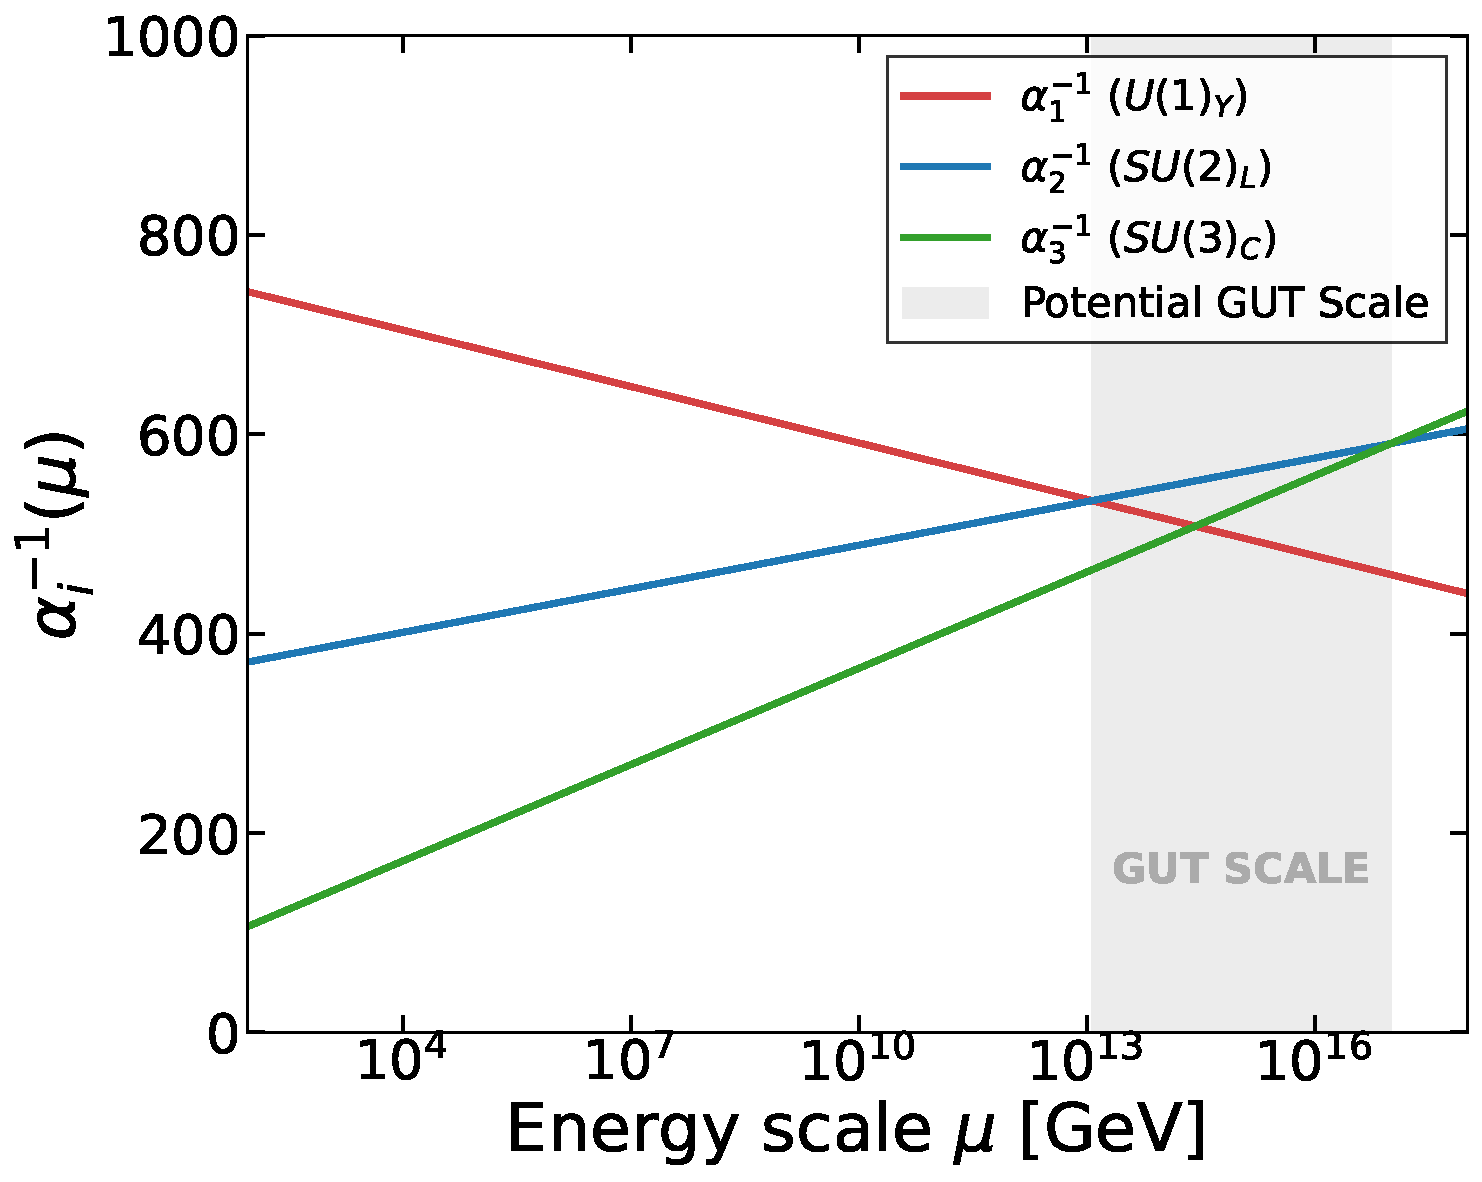
\includegraphics[width=\textwidth]{Figures/sm_unification.pdf}
        \caption{Inverse gauge coupling's dependence on energy scale} % 
        \label{fig:uni}
    \end{subfigure}
    \hspace{0.1cm}
    \begin{subfigure}[b]{0.49\textwidth}
        \centering
        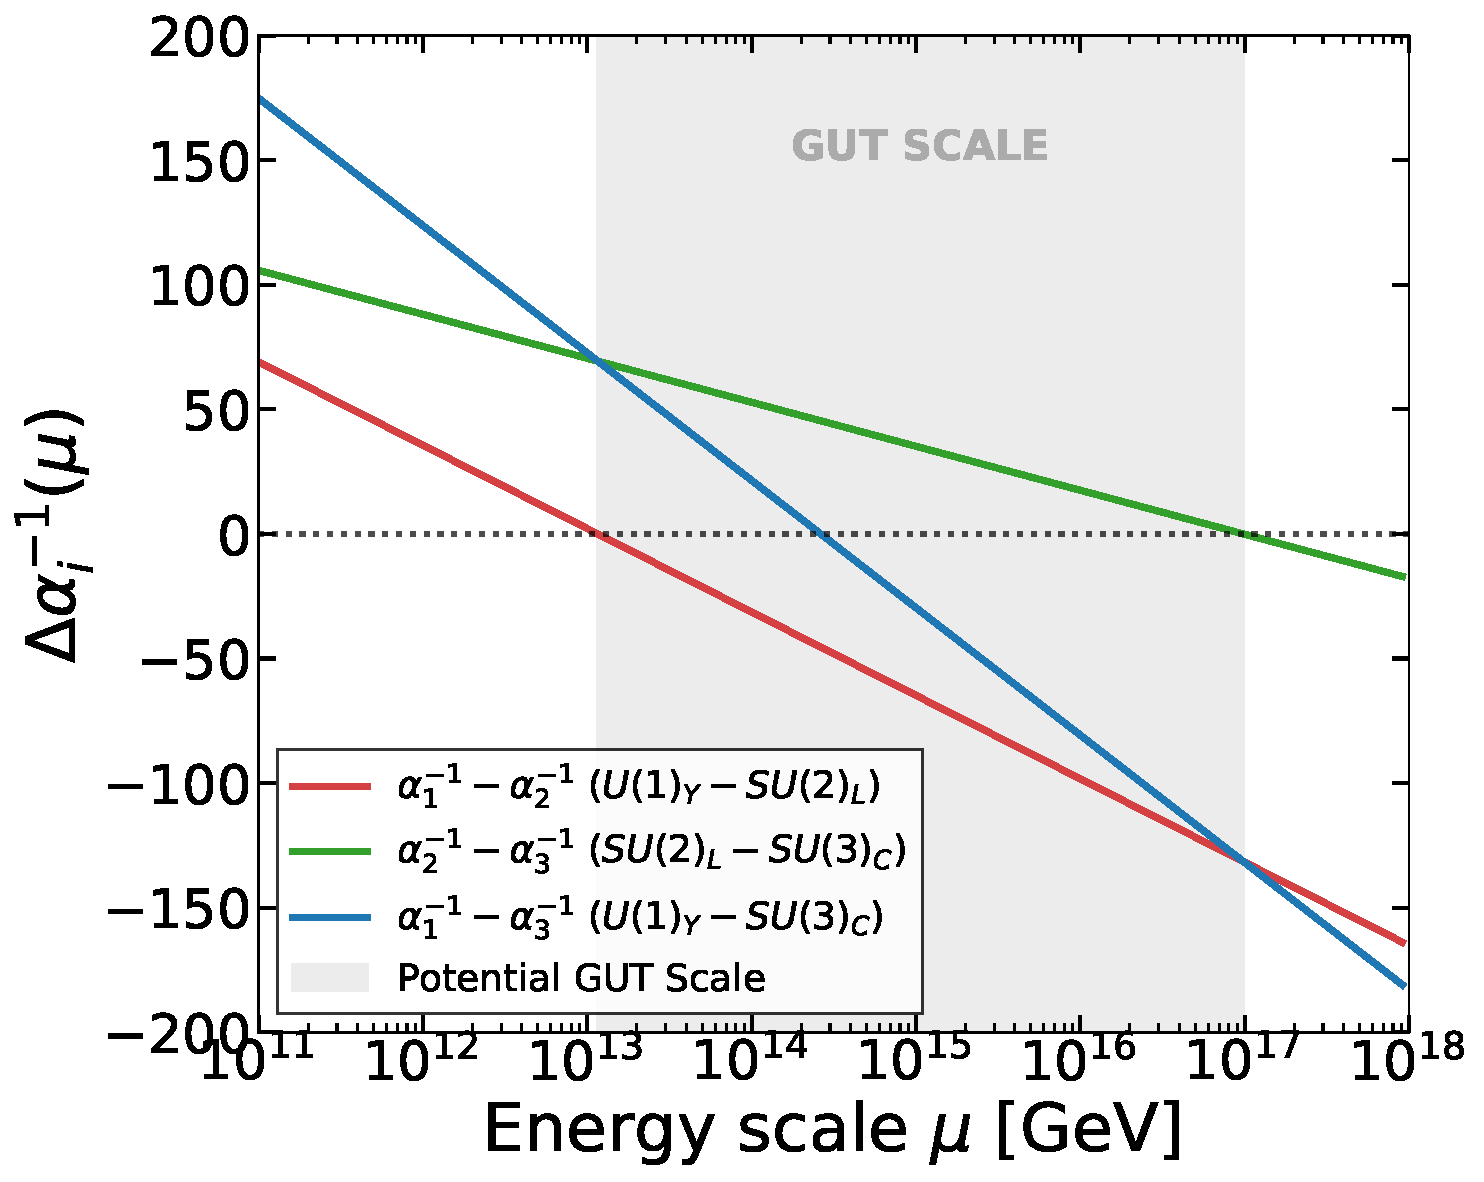
\includegraphics[width=\textwidth]{Figures/sm_unification_differences.pdf}
        \caption{Difference of gauge couplings} 
        \label{fig:uni_diff}
    \end{subfigure}
    \caption{The inverse gauge couplings (Eq. \eqref{eq:RGinversecoupling}) of $\U(1)_Y$ (red), $\SU(2)_L$ (blue), and $\SU(3)_C$ (green) are plotted in (a) against the energy scale in GeV. In (b) the difference of the couplings are shown, where the intersection with zero shows the intersection of (a). }
    \label{fig:SM_unification}
\end{figure}

We define a GUT to be a simple unifying group. However, there are also plenty of examples of product groups as unifying theories. A GUT has two main criteria: It needs to contain the SM gauge sector as a subgroup, and it must have complex representations such that the chiral structure of the SM can be reproduced \cite{Croon:2019kpe}. 

The model we will consider here is the first attempt of unifying the SM, namely the model proposed by H. Georgi and S. Glashow back in 1974 \cite{Georgi:1974yf}. This model is based on the smallest simple group $\SU(5)$, which contains the SM as a subgroup and has complex representations. 

\section{SU(5)}\label{sec:SU5}
\comment{OBS! Make the notation of the particles match the previous section (u,d,e,v vs u,d,Q,L)...}
To consider a possible simple group, which contains the SM gauge sector $\mathrm{SU}(3)_c\times\mathrm{SU}(2)_L\times\mathrm{U}(1)_Y$ as a subgroup, the rank of the group must be at least four, since $\SU(3)_c$ has rank $2$, $\SU(2)_L$ has rank $1$, $\U(1)_Y$ has rank $1$ as well. The simplest group that does this and has complex representations is $\SU(5)$ \cite{Georgi:1999wka}
\begin{equation}
    \mathrm{SU}(3)\times\mathrm{SU}(2)\times\mathrm{U}(1)\subset \mathrm{SU}(5)\,.
\end{equation}
Consider first the particles of the right-handed sector of the SM
\begin{equation}
    u_R^i : (\mathbf{3}, \mathbf{1})_{2/3} \,,\quad 
    d_R^i : (\mathbf{3}, \mathbf{1})_{-1/3} \,,\quad 
    \ell_R^i : (\mathbf{1}, \mathbf{1})_{-1} \,,\quad 
    (Q_L^i)^c : (\bar{\mathbf{3}}, \mathbf{2})_{-1/6} \,,\quad 
    (L_L^i)^c : (\mathbf{1}, \mathbf{2})_{1/2} \,, \label{eq:RparticlesSM}
\end{equation}
where the $c$ indicates the charge conjugated, and $i$ the generation. These particles represent the up quark, down quark, electron, anti-quarks and anti-leptons and can be found in Table \ref{tab:SMparticle}. These representations can be added through a direct sum
\begin{align}
    (3,1)_{2/3}\oplus (3,1)_{-1/3}\oplus (1,1)_{-1}\oplus(\bar{3},2)_{-1/6}\oplus(1,2)_{1/2} \,,
\end{align}
where we can write the complex conjugate of this expression as
\begin{align}
    (\bar{3},1)_{-2/3}\oplus (\bar{3},1)_{1/3}\oplus  (1,1)_{1}\oplus(3,2)_{1/6}\oplus(1,2)_{-1/2} \,.
\end{align}
It has been used that the $\SU(2)_L$ representation is real \cite{Georgi:1999wka}. 

The $\SU(5)$ group has two five-dimensional representations, namely $\bar{\mathbf{5}}$ and $\mathbf{5}$. Thus, we need to determine if the right-handed particles of the SM in Eq. \eqref{eq:RparticlesSM} can be grouped such that they fit in the $\mathbf{5}$ or $\bar{\mathbf{5}}$ multiplet of the $\SU(5)$ group. It is necessary to examine whether the generator of the $\U(1)_Y$ group $Y$ remains traceless\footnote{All the $\SU(N)$ groups are "special" groups, which means that the trace of the generators must be 0. However, the Abelian group $\U(1)_Y$ in the SM is not special and ensuring that the trace of the generator is zero is non-trivial. }. 

To build a $5\times 5$ matrix, we have two options
\begin{align}
    (3,1)_{2/3}\oplus(1,2)_{1/2}\,,\quad\text{or} \quad  (3,1)_{-1/3}\oplus(1,2)_{1/2}\,.\label{eq:irreps5}
\end{align}
To determine whether the combination is valid, we consider the trace of the generator $Y$ for the first option
\begin{align}
    \tr(S)=\tr\begin{pmatrix}
        \frac{2}{3}&0&0&0&0\\
        0&\frac{2}{3}&0&0&0\\
        0&0&\frac{2}{3}&0&0\\
        0&0&0&\frac{1}{2}&0\\
        0&0&0&0&\frac{1}{2}\\
    \end{pmatrix}=3\,.
\end{align}
Since this is not zero, this is not an option. The other case, however, evaluates to zero $(-1/3-1/3-1/3+1/2+1/2=0)$. The $\mathbf{5}$ can now be written as a column vector in terms of the particles of the SM from Eq. \eqref{eq:RparticlesSM}, it will consists of 
\begin{equation}
    \mathbf{5}\leftrightarrow \begin{pmatrix}
        d_1^\dagger\\d_2^\dagger\\d_3^\dagger\\\bar{e} ^\dagger\\\bar{\nu}^\dagger 
    \end{pmatrix}\,. \label{eq:5rep}
\end{equation}
The remaining particles from Eq. \eqref{eq:RparticlesSM} are 
\begin{equation}
     (3,1)_{2/3}\oplus (1,1)_{-1}\oplus(\bar{3},2)_{-1/6} \,,
     \label{eq:5repSU5}
\end{equation}
resulting in a ten-dimensional representation. $\SU(5)$ has two ten-dimensional representations $\overline{\mathbf{10}}$ and $\mathbf{10}$. This can be found by constructing the Young tableau of different direct products of representations of the group (see Appendix \ref{app:youngtab} and \ref{app:youngtabSUN}). We can construct the ten-representation by utilising the product of two fives
\begin{align}
    \mathbf{5} \otimes \mathbf{5} &= \mathbf{15} \oplus \mathbf{10} \,, \\[0.5ex] 
    \vcenter{\hbox{\ydiagram{1}}} \otimes \vcenter{\hbox{\ydiagram{1}}} &= \vcenter{\hbox{\ydiagram{2}}} \oplus \vcenter{\hbox{\ydiagram{1,1}}}\,.
\end{align}
As seen from the computation the symmetric part of the direct product is a $\mathbf{15}$ representation. Thus, we can take the anti-symmetric product of Eq. \eqref{eq:5repSU5} with itself to obtain the $\mathbf{10}$ representation \comment{expand the calulcation like down below}
\begin{align}
    \left[(3,1)_{-1/3}\oplus(1,2)_{1/2}\right]\otimes \left[(3,1)_{-1/3}\oplus(1,2)_{1/2}\right]_{AS}=\left[(\bar{3},1)_{-2/3}\oplus(1,1)_{1}\oplus(3,2)_{1/6}\right]\label{eq:irreps10}
\end{align}
where the hypercharge simply add \cite{Georgi:1999wka}. This gives us the complete conjugate of remaining particles from Eq. \eqref{eq:RparticlesSM}. We can thus write the remaining particles as the $\overline{\mathbf{10}}$ representation.
\begin{align}
\bar{\mathbf{10}} \leftrightarrow 
\begin{pmatrix}
    0 & u_3^\dagger & -u_2^\dagger & \bar{u}^{1\dagger} & \bar{d}^{1\dagger} \\
    -u_3^\dagger & 0 & u_1^\dagger & \bar{u}^{2\dagger} & \bar{d}^{2\dagger} \\
    u_2^\dagger & -u_1^\dagger & 0 & \bar{u}^{3\dagger} & \bar{d}^{3\dagger} \\
    -\bar{u}^{1\dagger} & -\bar{u}^{2\dagger} & -\bar{u}^{3\dagger} & 0 & e^\dagger \\
    -\bar{d}^{1\dagger} & -\bar{d}^{2\dagger} & -\bar{d}^{3\dagger} & -e^\dagger & 0
\end{pmatrix}\,,\label{eq:10barrep}
\end{align}
where $u_a^\dagger$ is right-handed up quarks, $\bar{u}_a^\dagger$ the right-handed anti-up quark, $\bar{d}_a^\dagger$ the right-handed anti-down quark, and $e^\dagger$ is right-handed electrons, where the index $a=1,2,3$ and describes the three colours.   
Note that the anti-symmetric part also ensures that the diagonal entries are trivial and thus that a particle cannot interact with itself. This removes five degrees of freedom from the twenty-five of the $5\times 5$ matrix. Furthermore, the definition of an anti-symmetric matrix also ensures that the entries are mirrored around the diagonal, leaving us with ten degrees of freedom, equal to the ten particles we had yet to describe. Thus, the two representations $\mathbf{5}$ (Eq. \eqref{eq:5rep}) and $\overline{\mathbf{10}}$ (Eq. \eqref{eq:10barrep}) hold all the particles of the SM (seen in Table \ref{tab:SMparticle}).
The same analysis can be done with the left-handed particles, which leaves one with the following representations 
\begin{align}
    \bar{\mathbf{5}}\leftrightarrow \begin{pmatrix}
        \bar{d}_1 \\ \bar{d}_2 \\ \bar{d}_3 \\ e \\ -\nu 
    \end{pmatrix}\quad \mathbf{10}\leftrightarrow \begin{pmatrix}
    0 & \bar{u}_3 & -\bar{u}_2 & u_1 & d_1 \\
    -\bar{u}_3 & 0 & \bar{u}_1 & u_2 & d_2 \\
    \bar{u}_2 & -\bar{u}_1 & 0 & u_3 & d_3 \\
    -u_1 & -u_2 & -u_3 & 0 & \bar{e} \\
    -d_1 & -d_2 & -d_3 & -\bar{e} & 0
\end{pmatrix}
\end{align} 
\subsection{Breaking of the GUT group to the SM gauge groups}
For $\SU(5)$ to be a valid GUT, we need a way of breaking the simple group down to the gauge sector of the SM $\mathrm{SU}(3)\times\mathrm{SU}(2)\times\mathrm{U}(1)$. The $\SU(5)$ group has $N^2-1=24$ gauge bosons, which transforms under the adjoint representation $\mathbf{24}$. The decomposition of this representation into irreducible representations (irreps) (see Appendix \ref{app:repersentations}) SM gauge group can be found by computing
\begin{align}
    \mathbf{5}\otimes\overline{\mathbf{5}}-1_{\SU(5)}\,,
\end{align}
using Eq. \eqref{eq:5rep}, we can write this as 
\begin{align}
    \left[(3,1)_{-1/3}\oplus(1,2)_{1/2}\right]\otimes \left[(\bar{3},1)_{1/3}\oplus(1,2)_{-1/2}\right]-(1,1)_0\,.
\end{align}
To compute this, we use the fact that the hypercharges add. There is only two non-trivial direct products that we have to compute, we will do these explicit. The first one is given by
\begin{align}
    (3,1)_{-1/3}\otimes(\bar{3},1)_{1/3}=(3\otimes\bar{3},1\otimes1)_0=(1,1)_0+(8,1)_0\,,
\end{align}
where
\begin{align}
    (3\otimes{\bar{3}})_{\SU(3)}=\vcenter{\hbox{\ydiagram{1}}} \otimes \vcenter{\hbox{\ydiagram{1,1}}}=\vcenter{\hbox{\ydiagram{1,1,1}}}\oplus \vcenter{\hbox{\ydiagram{2,1}}}\,,
\end{align}
where the $(1,1,1)$ Young tableau is the $\mathbf{1}$ representation, and $(2,1)$ is the $\mathbf{8}$ representation. The other non-trivial term is
\begin{align}
    (1,2)_{1/2}\otimes(1,2)_{-1/2}=(1\otimes1,2\otimes2)_0=(1,1)_0+(1,3)_0\,,
\end{align}
where
\begin{align}
    (2\otimes2)_{\SU(2)}=\vcenter{\hbox{\ydiagram{1}}} \otimes \vcenter{\hbox{\ydiagram{1}}}=\vcenter{\hbox{\ydiagram{1,1}}}\oplus \vcenter{\hbox{\ydiagram{2}}}\,,
\end{align}
where the $(1,1)$ Young tableau is the $1$ representation, and $(2)$ is the $3$ representation. Putting all the terms together, we obtain
\begin{align}
    \mathbf{24}\leftrightarrow (8,1)_0\oplus(1,3)_0\oplus(1,1)_0\oplus (3,2)_{-5/6}\oplus(\bar{3},2)_{5/6}\,. \label{eq:24irrep}
\end{align}
The field content of the adjoint representation of $\SU(5)$ is summarised in Table \ref{tab:adjSU5}. The first three terms in Eq. \eqref{eq:24irrep} is gauge bosons known from the SM (see Table \ref{tab:SMparticle}). The last two terms are however gauge bosons which are not a part of the SM. These force carriers is thus particles, which gain mass at the GUT scale through SSB, and therefore have not been observed experimentally. 
\begin{table}[ht]
\centering
\renewcommand{\arraystretch}{1.4}

\begin{tabularx}{\textwidth}{@{} >{\centering\arraybackslash}X >{\centering\arraybackslash}X >{\centering\arraybackslash}X @{}}
\toprule
\multicolumn{1}{c}{} & \multicolumn{1}{c}{\textbf{Part of the SM}} & \multicolumn{1}{c}{\textbf{Identification}} \\
\midrule
$(8,1)_0$           & \checkmark  & $G_\beta^\alpha$ \\
$(1,3)_0$           & \checkmark  & $W^\pm, W^0$ \\
$(1,1)_0$           & \checkmark  & B \\
$(3,2)_{-5/6}$      & X & $A_\alpha^\tau = (X_\alpha, Y_\alpha)$ \\
$(\bar{3},2)_{5/6}$ & X & $A_\tau^\alpha = (X_\alpha, Y_\alpha)^T$ \\
\bottomrule
\end{tabularx}
\caption{Gauge boson of the $\SU(5)$ GUT from the $24$ representation (Eq. \eqref{eq:24irrep}) and their identifications.}
\label{tab:adjSU5}
\end{table}

We can understand the SSB by writing the adjoint representation as a matrix using the generator $t^a$ 
\begin{align}
    \Phi=\phi^at^a\,,
\end{align}
where $a=1,2,\dots,24$ is the adjoint index \cite{Pernow:2021fvb}. Thus, the adjoint representation can be expressed as
\begin{equation}
    \Phi=\begin{pmatrix}
        A_{3\times3}&B_{3\times 2}\\
        C_{2\times3}&D_{2\times 2}
    \end{pmatrix}\,,
\end{equation}
where the subscript refers to the dimension of the submatrix. The upper left submatrix $A_{3\times3}$ acts like the strong force, $D_{2\times2}$ is equivalent to the weak force, and $B_{3\times2}$ and $C_{2\times3}$ mixes the strong and the weak force and are generally called the $X$ and $Y$ bosons, these are the ones which will eat the Goldstone bosons and require mass \cite{Peskin:1995ev}. 

The breaking of the $\SU(5)$ group is done analogously to the Higgs mechanism of the SM \cite{Pernow:2021fvb}. A scalar field transforming in the adjoint representation of the gauge group acquires a VEV. In this breaking we do not wish to break down the gauge structure of the SM. Thus the VEV needs to commute with the generators of $\mathcal{G}_{\mathrm{SM}}$. It is therefore useful to take a VEV which is proportional to the traceless $Y$ generator \cite{Georgi:1999wka}.    

To understand the SSB of $\SU(5)$, we consider the general renormalisable potential for the adjoint scalar
\begin{align}
    V=-\mu_1^3\tr\Phi-\mu_2^2\tr\Phi^2-\mu_3\tr\Phi^3+\lambda_1(\tr\Phi^2)^2+\lambda_2\tr\Phi^4\,,
\end{align}
where we can simplify the potential using that the generators $t^a$ of $\SU(N)$ are traceless and that we can impose parity symmetry. This yields
\begin{align}
    V=-\mu^2\tr\Phi^2+\lambda_1(\tr\Phi^2)^2+\lambda_2\tr\Phi^4\,.\label{eq:SU5pot}
\end{align}

We can now find a VEV of the potential. However, we must ensure that it commutes with the $Y$ generator. For convenience we consider $(-6)$ times the hypercharge
\begin{align}
    \langle\Phi\rangle=v\,\mathrm{diag}(2,2,2,-3,-3)\,.\label{eq:VEVdiag}
\end{align}
Before specifying the value of $v$, we first need to constrain our values of $\lambda_1,\,\lambda_2$ by considering all possible breaking of $\SU(5)$ \comment{check Peskin exercise}
\begin{align*}
    &\begin{pmatrix} a & & & & \\ & a & & & \\ & & a & & \\ & & & b & \\ & & & & b \end{pmatrix} \to \begin{matrix} 3a + 2b = 0 \\ \SU(3) \times \SU(2) \end{matrix} 
    & \begin{pmatrix} a & & & & \\ & b & & & \\ & & c & & \\ & & & d & \\ & & & & e \end{pmatrix} \to \begin{matrix} a+b+c+d+e = 0 \\ \U(1)\times \U(1)\times\U(1)\times\U(1)\times\U(1) \end{matrix} \\[15pt]
    &\begin{pmatrix} a & & & & \\ & a & & & \\ & & a & & \\ & & & a & \\ & & & & b \end{pmatrix} \to \begin{matrix} 4a + b = 0 \\ SU(4) \times U(1) \end{matrix} 
    &\begin{pmatrix} a & & & & \\ & a & & & \\ & & a & & \\ & & & b & \\ & & & & c \end{pmatrix} \to \begin{matrix} 3a + b + c = 0 \\ SU(3) \times U(1) \times U(1) \end{matrix} \\[15pt]
    &\begin{pmatrix} a & & & & \\ & a & & & \\ & & b & & \\ & & & b & \\ & & & & c \end{pmatrix} \to \begin{matrix} 2(a + b) + c = 0 \\ SU(2) \times SU(2) \times U(1) \end{matrix} 
    &\begin{pmatrix} a & & & & \\ & a & & & \\ & & b & & \\ & & & c & \\ & & & & d \end{pmatrix} \to \begin{matrix} 2a + b + c + d = 0 \\ SU(2) \times U(1) \times U(1) \times U(1) \end{matrix}
\end{align*}
As already noted, the desired breaking is the first which successfully breaks $\SU(5)$ to the SM. To ensure this is the VEV the model actually realises, we need to ensure that it is the minimal VEV. In general, when theories break down to more complex group structures, the VEV becomes larger. We can thus focus on the two simplest sets of eigenvalues, where there are only two variables. First, we can write the derivative of the potential (Eq. \eqref{eq:SU5pot}) in a general form
\begin{align}
    \frac{\partial V}{\partial v}=-2\mu^2 v A+4v^3(\lambda_1A^2+\lambda_2B)\,,
\end{align}
where $A=\tr\Phi^2/v^2$ and $B=\tr\Phi^4/v^4$. If we now minimise the potential, the expression for $v^2$ yields
\begin{align}
    v^2=\frac{\mu^2 A}{2(\lambda_1A^2+\lambda_2B)} \label{eq:VEVvalue}
\end{align}
Let us plug this back into the potential Eq. \eqref{eq:SU5pot} and simplify 
\begin{align}
    V_{\min}&=-\mu^2A\frac{\mu^2 A}{2(\lambda_1A^2+\lambda_2B)}+\lambda_1A^2\left(\frac{\mu^2 A}{2(\lambda_1A^2+\lambda_2B)}\right)^2+\lambda_2B\left(\frac{\mu^2 A}{2(\lambda_1A^2+\lambda_2B)}\right)^2\nonumber
    \\
    &=-\frac{\mu^4 A^2}{2(\lambda_1A^2+\lambda_2B)}+\lambda_1\frac{\mu^4 A^4}{4(\lambda_1A^2+\lambda_2B)^2}+\lambda_2\frac{\mu^4 A^2B}{4(\lambda_1A^2+\lambda_2B)^2}\nonumber
    \\
    &=\frac{-2(\lambda_1A^2+\lambda_2B)\mu^4 A^2+\mu^4 A^4\lambda_1+\mu^4 A^2B\lambda_2}{4(\lambda_1A^2+\lambda_2B)^2}\nonumber
     \\
    &=\frac{-\mu^4A^2}{4(\lambda_1A^2+\lambda_2B)^2}\left[2(\lambda_1A^2+\lambda_2B)-A^2\lambda_1-B\lambda_2\right]\nonumber
    \\
    &=\frac{-\mu^4A^2}{4(\lambda_1A^2+\lambda_2B)}
\end{align}
Thus the minimal potential depends on $\lambda_{\text{eff}}$ as
\begin{align}
    V_{{\min}}\sim-\frac{\mu^4}{\lambda_{\text{eff}}}\,,\label{eq:1/lambdaeff}
\end{align}
where $\lambda_{\text{eff}}=\lambda_1+\lambda_2\frac{B}{A^2}$. 

To ensure that we obtain the $\SU(3) \times \SU(2)$ breaking rather than the $\SU(4) \times \U(1)$ breaking, we can compute the values of $A$ and $B$ in both cases. For the first case 
\begin{align}
    A_{(3,2)} &= \frac{\tr(\Phi^2)}{v^2} = 3a^2 + 2\left(-\frac{3}{2}a\right)^2 = \frac{15}{2} a^2 \,, \label{eq:VEVA_32} \\
    B_{(3,2)} &= \frac{\tr(\Phi^4)}{v^4} = 3a^4 + 2\left(-\frac{3}{2}a\right)^4 = \frac{105}{8} a^4 \,. \label{eq:VEVB_32}
\end{align}
where the condition $b=-\frac{3}{2}a$ has been used. In the second case, we obtain 
\begin{align}
    A_{(4,1)} &=  4a^2 + (-4a)^2 = 20a^2 \,, \label{eq:VEVA_41} \\
    B_{(4,1)} &= 4a^4 + (-4a)^4 = 260a^4 \,. \label{eq:VEVB_41}
\end{align}
where $b=-4a$ has been used. To ensure that the VEV is smaller in the case of $\SU(3) \times \SU(2)$ breaking, a boundary on the quartic coupling, using Eq. \eqref{eq:1/lambdaeff}, is obtained
\begin{align}
    V_{(3,2)}&<V_{(4,1)}\\
    \lambda_{\text{eff}_{(3,2)}}&<\lambda_{\text{eff}_{(4,1)}}
    \\\lambda_2 \frac{7}{30}&<\lambda_2\frac{13}{20}\,.
\end{align}
This is only the case for $\lambda_2>0$. 

Now to ensure a bounded potential from below, we also require $\lambda_{\text{eff}}>0$. From this, we obtain a boundary on $\lambda_1$
\begin{align}
    \lambda_{\text{eff}}&>0\\
    \lambda_1&>-\lambda_2\frac{7}{30}\,.
\end{align}
This effectively breaks down our gauge group from $\SU(5)\to\SU(3)\times\SU(2)\times\U(1)$, since $\U(1)_Y$ by construction commutes with the VEV. This ensures that the X and Y bosons gain mass at the GUT scale. After symmetry-breaking, eight of the twenty-four gauge bosons are the gluons, three are the weak gauge bosons, and one is the hypercharge gauge boson \cite{Pernow:2021fvb} as seen in Table \ref{tab:adjSU5}.

With the constraints on $\lambda_2$ and $\lambda_1$, the VEV can be found by combining Eqs. \eqref{eq:VEVvalue} and \eqref{eq:VEVdiag}
\begin{align}
    \langle \Phi\rangle=\frac{\mu^2}{2(30\lambda_1+7\lambda_2)}\mathrm{diag}(2,2,2,-3,-3)\,,
\end{align}
where the values of $A$ and $B$ are given by Eqs. \eqref{eq:VEVA_32} and \eqref{eq:VEVB_32}.

\subsection{The Higgs boson in SU(5)}
With the GUT broken down to the SM, the next step is to introduce a scalar field which can break the electroweak symmetry, playing the role of the Higgs boson in the SM. The Higgs transforms as $(1,2)_{\pm1/2}$ under $\mathcal{G}_\mathrm{SM}$. This scalar is required to  generate mass for the right-handed positron $(\bar{e})$ and the down type quarks $(d)$.  These specific states reside in the $\mathbf{5}$ representation (see Eq. \eqref{eq:5repSU5}), and their corresponding anti-particles in $\overline{\mathbf{10}}$ (see Eq. \eqref{eq:10barrep}). Their mass term must arise from the tensor product of these representations \cite{Georgi:1999wka}
\begin{align}
     (\overline{\mathbf{10}}\otimes{\mathbf{5}})_{\SU(5)}=\vcenter{\hbox{\ydiagram{1,1,1}}} \otimes \vcenter{\hbox{\ydiagram{1}}}=\vcenter{\hbox{\ydiagram{2,1,1}}}\oplus \vcenter{\hbox{\ydiagram{1,1,1,1}}} =\overline{\mathbf{45}}\otimes \overline{\mathbf{5}}\,, 
\end{align} 
Besides from the positron and down type quarks, the scalar must also generate masses for the ${u}$ and $\overline{u}$ states, both of which is contained in the $\overline{\mathbf{10}}$ representation. Let us consider the product of the representation with itself
\begin{align}
     (\overline{\mathbf{10}}\otimes{\overline{\mathbf{10}}})_{\SU(5)}&=\vcenter{\hbox{\ydiagram{1,1,1}}} \otimes \vcenter{\hbox{\ydiagram{1,1,1}}}\\&\implies
\begin{ytableau} ~ \\ ~ \\ ~ \end{ytableau} \otimes \begin{ytableau} a \\ b \\ c \end{ytableau} 
= \left(
\begin{ytableau} ~ \\ ~ \\ ~ \\ a \end{ytableau} \oplus 
\begin{ytableau} ~ & a \\ ~ \\ ~ \end{ytableau}
\right) \otimes \begin{ytableau} b \\ c \end{ytableau} 
= \left(
\begin{ytableau} ~ \\ ~ \\ ~ \\ a \\ b \end{ytableau} \oplus 
\begin{ytableau} ~ & a \\ ~ & b \\ ~ \end{ytableau} \oplus 
\begin{ytableau} ~ & a \\ ~ \\ ~ \\ b \end{ytableau}
\right) \otimes \begin{ytableau} c \end{ytableau} \\
&= \begin{ytableau} ~ \\ ~ \\ ~ \\ a \\ b \\ c \end{ytableau} \oplus 
\begin{ytableau} ~ & a \\ ~ & b \\ ~ \\ c \end{ytableau} \oplus 
\begin{ytableau} ~ & a \\ ~ & b \\ ~ & c \end{ytableau}=\begin{ytableau} ~ \\ \end{ytableau} \oplus 
\begin{ytableau} ~ & ~ \\ ~ & ~ \\ ~ \\ ~ \end{ytableau} \oplus 
\begin{ytableau} ~ & ~ \\ ~ & ~ \\ ~ & ~ \end{ytableau}={\mathbf{5}}\oplus {\mathbf{45}}\oplus {\mathbf{50}}
\end{align}
To determine the allowed representations, the decomposition of the representations need to contain a multiplet with the same quantum numbers of the SM Higgs $(1,2)_{\pm1/2}$. The Higgs like scalar can reside in either the ${\mathbf{5}}$ or ${\mathbf{45}}$ \cite{Georgi:1999wka} (see Eq. \eqref{eq:irreps5} for the ${\mathbf{5}}$ representation). To confirm that this is also the case for the ${\mathbf{45}}$ representation we can compute the direct product of the two representations ${\mathbf{5}}\otimes\overline{{\mathbf{10}}}$. We will demonstrate this by utilising the decomposition in Eq. \eqref{eq:irreps5} and \eqref{eq:irreps10}, which yields
 \begin{align}
    &\left( (3,1)_{-1/3} \oplus (1,2)_{1/2} \right) \otimes \left( (3,1)_{2/3} \oplus (1,1)_{-1} \oplus (\bar{3},2)_{-1/6} \right) \\&= (6,1)_{1/3} \oplus (\bar{3},1)_{1/3} \oplus (3,1)_{-4/3} \oplus (\bar{8},2)_{-1/2} \oplus (1,2)_{-1/2} \nonumber\\&\quad\oplus (3,2)_{7/6} \oplus (1,2)_{-1/2}\oplus (\bar{3},3)_{1/3}\oplus (\bar{3},1)_{1/3}\,.
\end{align}
We can now remove the irreps which make out the $\mathbf{5}$ representations (see Eq. \eqref{eq:irreps5}), effectively revealing the decomposition of the $\mathbf{45}$ representation
 \begin{align}
    \mathbf{45}\leftrightarrow&\left( (3,1)_{-1/3} \oplus (1,2)_{1/2} \right) \otimes \left( (3,1)_{2/3} \oplus (1,1)_{-1} \oplus (\bar{3},2)_{-1/6} \right) \\&= (6,1)_{1/3} \oplus (\bar{3},1)_{1/3} \oplus (3,1)_{-4/3} \oplus (\bar{8},2)_{-1/2} \oplus (1,2)_{-1/2} \oplus (3,2)_{7/6} \oplus (\bar{3},3)_{1/3}\,,
\end{align}
which includes the Higgs like irrep $(1,2)_{-1/2} $. Thus both ${\mathbf{5}}$ or ${\mathbf{45}}$ can be used to introduce a Higgs like scalar into the GUT.  

While conceptually compelling, the minimal $\SU(5)$ model encounters fundamental issues. A theoretical limitation of the model is the so-called \textit{doublet-triplet splitting} \cite{Croon:2019kpe}. This issue arises from the embedding the Higgs scalar within the $\mathbf{5}$ representation. This choice requires fine-tuning of the masses of the multiplets coloured components compared to the uncoloured components. The colour-triplet states needs to be heavy (around GUT scale) to avoid proton decay with a low decay rate. In contrast to the uncoloured doublet needs to be relatively light to ensure that the Higgs mass is in agreement with the measured mass of the Higgs $m_H=125.18\,$GeV \cite{Croon:2019kpe}. 

A further shortcoming of the model is its lack of generating neutrino mass. Different attempts to fix this have been proposed see \cite{FileviezPerez:2007bcw, Zee:1980ai,FileviezPerez:2016sal}. 

Lastly, the biggest challenge of the model is its prediction of rapid proton decay. The mixing of quarks and leptons in the representations successfully explains the neutralness of the atom. However, this mixing also results the $X$ and $Y$ gauge bosons, which mediate the proton decay and estimates the proton lifetime at \cite{Croon:2019kpe}
\begin{align}
    \tau_p\sim\frac{M_X^4}{m_p^5}\,,
\end{align}
where $m_p$ is the mass of the proton and $M_X$ is the scale of unification. As seen in Figures \ref{fig:uni} above, the assumed unification scale is around $\mu\sim10^{15}\,$GeV. This results in a proton decay rate of $\sim10^{31}\,$years. Since proton decay has not (yet) been observed, there is an experimental lower bound on the decay time of proton at the order of $10^{34}\,$years \cite{Takenaka:2020cmb}. This bound is the results of the experiment the Super-Kamiokande and is thus in disagreement with the estimate from the $\SU(5)$ GUT. Changes to the Higgs sector of the model can help this problem, see \cite{Dorsner:2005fq,Dorsner:2006dj,Fornal:2017xcj,FileviezPerez:2018dyf}. 

\section{Alternative GUTs}
The unification of the SM gauge groups does not necessarily need to be restricted to be the simplest embedding. Investigating larger symmetry groups provides alternative frameworks, with on of them being the $\mathrm{SO}(10)$ group. This group has the $\SU(5)$ GUT as a subgroup \cite{Georgi:1999wka}
\begin{equation}
    \mathrm{SU}(5)\times \U (1)\subset \mathrm{SO}(10)\,.
\end{equation}
The $\SO (10)$ GUT also suffer from the prediction of proton decay, however it resolves several of $\SU(5)$'s issues. Most notably, the $\SO(10)$ generates neutrino masses, through the inclusion of a right-handed neutrino. Furthermore, it fits the entire particle content of the SM into one single $\mathbf{16}$ representation \cite{Fritzsch:1974nn}. 

Besides the $\SU (5)$ and $\SO(10)$ GUTs, there are multiple other possibilities, such as the exceptional Lie group \cite{Gursey:1975ki}
\begin{equation}
    \SU(5)\subset\SO(10)\subset\E_6\,.
\end{equation}
This embedding of the SM is particularly studied within the string theory community, because the group structure of $\E_6$ is a subgroup of $\E_8\times\E_8$, which is the group structure of \textit{heterotic string theory} \cite{Witten:1985xc,Candelas:1985en}. This would essentially introduce a possible theory of everything, which would break down to an $\E_6$ GUT. This model, however, suffers from a large fundamental representation of $\mathbf{27}$, which introduces a lot of new particles, besides the particles from the SM. Furthermore, the Higgs sector is based on large representations and the breaking of the model down to the SM introduces an extra gauge boson, which has not been discovered experimentally \cite{Langacker:2008yv}. 

Another set of models are semi-simple groups, such as Pati--Salam \cite{Pati:1974yy} $\SU(4)_C\times \SU(2)_L\times\SU(2)_R$. This GUT restores the left-right symmetry at high energies and at low energies, the $\SU(2)_R$ is broken, ensuring the left-handed bias that we have in the SM. Additionally, it gauges the lepton number as a symmetry. 

Another semi-simple GUT is the so-called Flipped $\SU(5)$ \cite{Barr:1981qv,DeRujula:1980qc} which has the gauge structure $\SU(5)\times\U(1)$. This model solves the doublet-triplet splitting problem of the minimal $\SU(5)$ discussed above \cite{Croon:2019kpe}. 

Other models such as Trinification $\SU(3)\times\SU(3)\times\SU(3)$ has also been explored \cite{Achiman:1978rv}.

Despite the models individual shortcomings and differing particle additions, all GUTs share the same core requirements. They must include the necessary fermion generations, supply the scalar fields required to break the unified group down to the SM, and a scalar to play the role of the Higgs.

Another possibility is supersymmetric (SUSY) GUTs \cite{Dimopoulos:1981zb}. This introduces a symmetry between bosons and fermions, resulting in twice the number of particles in the SM. Every particle would have a supersymmetric counterpart; for instance: quarks would have \textit{squarks}, and leptons would have \textit{sleptons}. One of the models shortcomings is that none of the supersymmetric particles has been found yet. A quality of the SUSY GUT is that the Figure \ref{fig:uni} will change, and have an actual intersection of all three couplings at the SUSY GUT scale $10^{16}\,$GeV. This ensures a higher decay time for protons and thus the $\SU(5)$ GUT would not be ruled out based on the prediction of proton decay. 

In this thesis, we will focus on simple GUTs based on non-SUSY $\SU(N)$ groups. In the next chapter, we will explore \textit{complete asymptotic freedom} of the $\SU(N)$ groups.  
